\documentclass{standalone}
\usepackage{tikz}
\usetikzlibrary{patterns, positioning}

\begin{document}
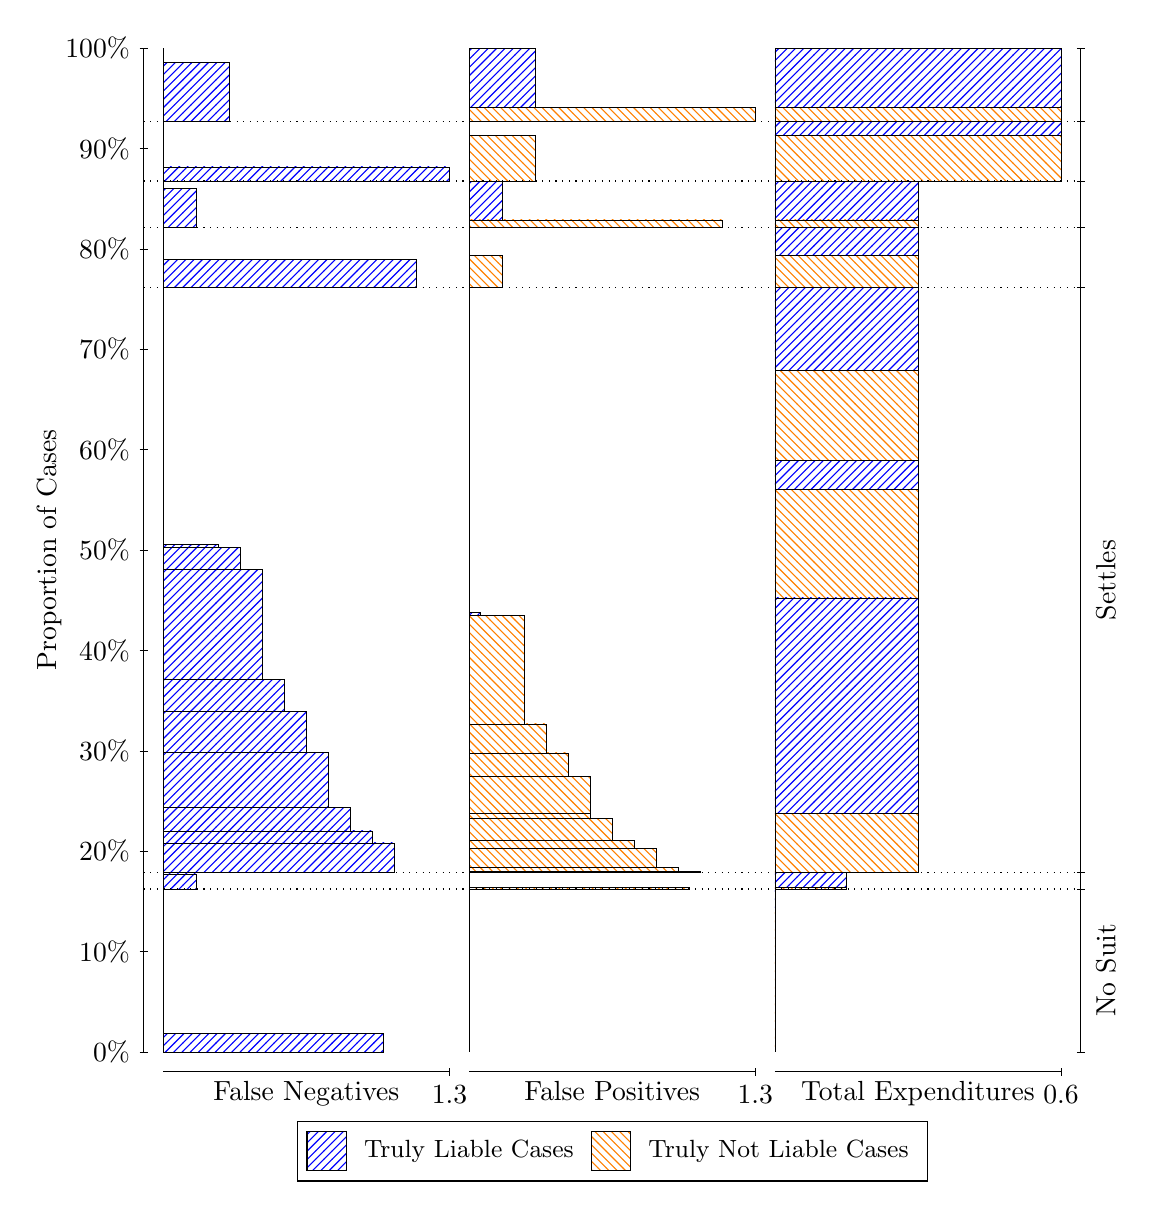
\begin{tikzpicture}
\draw[black, very thin] (1.5,1.75) -- (1.5,14.5);
\node[rotate=90, anchor=center] at (0.3, 8.125) {Proportion of Cases};
\draw[black, very thin] (1.45,1.75) -- (1.55,1.75);
\node[anchor=east] at (1.45, 1.75) {0\%};
\draw[black, very thin] (1.45,3.025) -- (1.55,3.025);
\node[anchor=east] at (1.45, 3.025) {10\%};
\draw[black, very thin] (1.45,4.3) -- (1.55,4.3);
\node[anchor=east] at (1.45, 4.3) {20\%};
\draw[black, very thin] (1.45,5.575) -- (1.55,5.575);
\node[anchor=east] at (1.45, 5.575) {30\%};
\draw[black, very thin] (1.45,6.85) -- (1.55,6.85);
\node[anchor=east] at (1.45, 6.85) {40\%};
\draw[black, very thin] (1.45,8.125) -- (1.55,8.125);
\node[anchor=east] at (1.45, 8.125) {50\%};
\draw[black, very thin] (1.45,9.4) -- (1.55,9.4);
\node[anchor=east] at (1.45, 9.4) {60\%};
\draw[black, very thin] (1.45,10.675) -- (1.55,10.675);
\node[anchor=east] at (1.45, 10.675) {70\%};
\draw[black, very thin] (1.45,11.95) -- (1.55,11.95);
\node[anchor=east] at (1.45, 11.95) {80\%};
\draw[black, very thin] (1.45,13.225) -- (1.55,13.225);
\node[anchor=east] at (1.45, 13.225) {90\%};
\draw[black, very thin] (1.45,14.5) -- (1.55,14.5);
\node[anchor=east] at (1.45, 14.5) {100\%};

\draw[black, very thin] (13.4,1.75) -- (13.4,14.5);
\draw[black, very thin] (13.35,1.75) -- (13.45,1.75);
\node[anchor=west] at (13.35, 1.75) {};
\draw[black, very thin] (13.35,3.8202) -- (13.45,3.8202);
\node[anchor=west] at (13.35, 3.8202) {};
\draw[black, very thin] (13.35,4.0323) -- (13.45,4.0323);
\node[anchor=west] at (13.35, 4.0323) {};
\draw[black, very thin] (13.35,11.457) -- (13.45,11.457);
\node[anchor=west] at (13.35, 11.457) {};
\draw[black, very thin] (13.35,12.222) -- (13.45,12.222);
\node[anchor=west] at (13.35, 12.222) {};
\draw[black, very thin] (13.35,12.811) -- (13.45,12.811);
\node[anchor=west] at (13.35, 12.811) {};
\draw[black, very thin] (13.35,13.57) -- (13.45,13.57);
\node[anchor=west] at (13.35, 13.57) {};
\draw[black, very thin] (13.35,14.5) -- (13.45,14.5);
\node[anchor=west] at (13.35, 14.5) {};

\draw[black, very thin, pattern color=blue, pattern=north east lines] (1.75,1.75) rectangle (4.5449,1.9903);
\draw[black, very thin, pattern color=orange, pattern=north west lines] (1.75,1.9903) rectangle (1.75,3.8202);
\draw[black, very thin, pattern color=blue, pattern=north east lines] (1.75,3.8202) rectangle (2.1692,4.0106);
\draw[black, very thin, pattern color=orange, pattern=north west lines] (1.75,4.0106) rectangle (1.75,4.0323);
\draw[black, very thin, pattern color=blue, pattern=north east lines] (1.75,4.0323) rectangle (4.6846,4.4055);
\draw[black, very thin, pattern color=blue, pattern=north east lines] (1.75,4.4055) rectangle (4.4051,4.5588);
\draw[black, very thin, pattern color=blue, pattern=north east lines] (1.75,4.5588) rectangle (4.1256,4.8554);
\draw[black, very thin, pattern color=blue, pattern=north east lines] (1.75,4.8554) rectangle (3.8462,5.5587);
\draw[black, very thin, pattern color=blue, pattern=north east lines] (1.75,5.5587) rectangle (3.5667,6.0787);
\draw[black, very thin, pattern color=blue, pattern=north east lines] (1.75,6.0787) rectangle (3.2872,6.481);
\draw[black, very thin, pattern color=blue, pattern=north east lines] (1.75,6.481) rectangle (3.0077,7.8789);
\draw[black, very thin, pattern color=blue, pattern=north east lines] (1.75,7.8789) rectangle (2.7282,8.1544);
\draw[black, very thin, pattern color=blue, pattern=north east lines] (1.75,8.1544) rectangle (2.4487,8.1961);
\draw[black, very thin, pattern color=orange, pattern=north west lines] (1.75,8.1961) rectangle (1.75,11.457);
\draw[black, very thin, pattern color=blue, pattern=north east lines] (1.75,11.457) rectangle (4.9641,11.814);
\draw[black, very thin, pattern color=orange, pattern=north west lines] (1.75,11.814) rectangle (1.75,12.222);
\draw[black, very thin, pattern color=blue, pattern=north east lines] (1.75,12.222) rectangle (2.1692,12.717);
\draw[black, very thin, pattern color=orange, pattern=north west lines] (1.75,12.717) rectangle (1.75,12.811);
\draw[black, very thin, pattern color=blue, pattern=north east lines] (1.75,12.811) rectangle (5.3833,12.99);
\draw[black, very thin, pattern color=orange, pattern=north west lines] (1.75,12.99) rectangle (1.75,13.57);
\draw[black, very thin, pattern color=blue, pattern=north east lines] (1.75,13.57) rectangle (2.5885,14.32);
\draw[black, very thin, pattern color=orange, pattern=north west lines] (1.75,14.32) rectangle (1.75,14.5);
\draw[black, very thin, pattern color=orange, pattern=north west lines] (5.6333,1.75) rectangle (5.6333,3.5799);
\draw[black, very thin, pattern color=blue, pattern=north east lines] (5.6333,3.5799) rectangle (5.6333,3.8202);
\draw[black, very thin, pattern color=orange, pattern=north west lines] (5.6333,3.8202) rectangle (8.4282,3.8419);
\draw[black, very thin, pattern color=blue, pattern=north east lines] (5.6333,3.8419) rectangle (5.6333,4.0323);
\draw[black, very thin, pattern color=orange, pattern=north west lines] (5.6333,4.0323) rectangle (8.5679,4.0427);
\draw[black, very thin, pattern color=orange, pattern=north west lines] (5.6333,4.0427) rectangle (8.2885,4.0897);
\draw[black, very thin, pattern color=orange, pattern=north west lines] (5.6333,4.0897) rectangle (8.009,4.3377);
\draw[black, very thin, pattern color=orange, pattern=north west lines] (5.6333,4.3377) rectangle (7.7295,4.4418);
\draw[black, very thin, pattern color=orange, pattern=north west lines] (5.6333,4.4418) rectangle (7.45,4.7184);
\draw[black, very thin, pattern color=orange, pattern=north west lines] (5.6333,4.7184) rectangle (7.1705,4.7769);
\draw[black, very thin, pattern color=orange, pattern=north west lines] (5.6333,4.7769) rectangle (7.1705,5.2514);
\draw[black, very thin, pattern color=orange, pattern=north west lines] (5.6333,5.2514) rectangle (6.891,5.5494);
\draw[black, very thin, pattern color=orange, pattern=north west lines] (5.6333,5.5494) rectangle (6.6115,5.9169);
\draw[black, very thin, pattern color=orange, pattern=north west lines] (5.6333,5.9169) rectangle (6.3321,7.2934);
\draw[black, very thin, pattern color=blue, pattern=north east lines] (5.6333,7.2934) rectangle (5.7731,7.3351);
\draw[black, very thin, pattern color=blue, pattern=north east lines] (5.6333,7.3351) rectangle (5.6333,11.457);
\draw[black, very thin, pattern color=orange, pattern=north west lines] (5.6333,11.457) rectangle (6.0526,11.865);
\draw[black, very thin, pattern color=blue, pattern=north east lines] (5.6333,11.865) rectangle (5.6333,12.222);
\draw[black, very thin, pattern color=orange, pattern=north west lines] (5.6333,12.222) rectangle (8.8474,12.317);
\draw[black, very thin, pattern color=blue, pattern=north east lines] (5.6333,12.317) rectangle (6.0526,12.811);
\draw[black, very thin, pattern color=orange, pattern=north west lines] (5.6333,12.811) rectangle (6.4718,13.392);
\draw[black, very thin, pattern color=blue, pattern=north east lines] (5.6333,13.392) rectangle (5.6333,13.57);
\draw[black, very thin, pattern color=orange, pattern=north west lines] (5.6333,13.57) rectangle (9.2667,13.75);
\draw[black, very thin, pattern color=blue, pattern=north east lines] (5.6333,13.75) rectangle (6.4718,14.5);
\draw[black, very thin, pattern color=orange, pattern=north west lines] (9.5167,1.75) rectangle (9.5167,3.5799);
\draw[black, very thin, pattern color=blue, pattern=north east lines] (9.5167,3.5799) rectangle (9.5167,3.8202);
\draw[black, very thin, pattern color=orange, pattern=north west lines] (9.5167,3.8202) rectangle (10.425,3.8419);
\draw[black, very thin, pattern color=blue, pattern=north east lines] (9.5167,3.8419) rectangle (10.425,4.0323);
\draw[black, very thin, pattern color=orange, pattern=north west lines] (9.5167,4.0323) rectangle (11.333,4.7769);
\draw[black, very thin, pattern color=blue, pattern=north east lines] (9.5167,4.7769) rectangle (11.333,7.5159);
\draw[black, very thin, pattern color=orange, pattern=north west lines] (9.5167,7.5159) rectangle (11.333,8.8923);
\draw[black, very thin, pattern color=blue, pattern=north east lines] (9.5167,8.8923) rectangle (11.333,9.2655);
\draw[black, very thin, pattern color=orange, pattern=north west lines] (9.5167,9.2655) rectangle (11.333,10.406);
\draw[black, very thin, pattern color=blue, pattern=north east lines] (9.5167,10.406) rectangle (11.333,11.457);
\draw[black, very thin, pattern color=orange, pattern=north west lines] (9.5167,11.457) rectangle (11.333,11.865);
\draw[black, very thin, pattern color=blue, pattern=north east lines] (9.5167,11.865) rectangle (11.333,12.222);
\draw[black, very thin, pattern color=orange, pattern=north west lines] (9.5167,12.222) rectangle (11.333,12.317);
\draw[black, very thin, pattern color=blue, pattern=north east lines] (9.5167,12.317) rectangle (11.333,12.811);
\draw[black, very thin, pattern color=orange, pattern=north west lines] (9.5167,12.811) rectangle (13.15,13.392);
\draw[black, very thin, pattern color=blue, pattern=north east lines] (9.5167,13.392) rectangle (13.15,13.57);
\draw[black, very thin, pattern color=orange, pattern=north west lines] (9.5167,13.57) rectangle (13.15,13.75);
\draw[black, very thin, pattern color=blue, pattern=north east lines] (9.5167,13.75) rectangle (13.15,14.5);
\draw[black, dotted] (1.5,3.8202) -- (13.4,3.8202);
\draw[black, dotted] (1.5,4.0323) -- (13.4,4.0323);
\draw[black, dotted] (1.5,11.457) -- (13.4,11.457);
\draw[black, dotted] (1.5,12.222) -- (13.4,12.222);
\draw[black, dotted] (1.5,12.811) -- (13.4,12.811);
\draw[black, dotted] (1.5,13.57) -- (13.4,13.57);
\draw[black, very thin] (1.75,1.5) -- (5.3833,1.5);
\node[anchor=north] at (3.5667, 1.5) {False Negatives};
\draw[black, very thin] (5.3833,1.45) -- (5.3833,1.55);
\node[anchor=north] at (5.3833, 1.45) {1.3};

\draw[black, very thin] (5.6333,1.5) -- (9.2667,1.5);
\node[anchor=north] at (7.45, 1.5) {False Positives};
\draw[black, very thin] (9.2667,1.45) -- (9.2667,1.55);
\node[anchor=north] at (9.2667, 1.45) {1.3};

\draw[black, very thin] (9.5167,1.5) -- (13.15,1.5);
\node[anchor=north] at (11.333, 1.5) {Total Expenditures};
\draw[black, very thin] (13.15,1.45) -- (13.15,1.55);
\node[anchor=north] at (13.15, 1.45) {0.6};

\node[black, centered, rotate=90] at (13.72, 2.7851) {No Suit};

\node[black, centered, rotate=90] at (13.72, 7.7447) {Settles};





\draw (7.449999999999999,1.5) node[draw=none] (baseCoordinate) {};
\begin{scope}[align=center]
        \matrix[scale=0.5, draw=black, below=0.5cm of baseCoordinate, nodes={draw}, column sep=0.1cm]{
            \node[rectangle, draw, minimum width=0.5cm, minimum height=0.5cm, pattern=north east lines, pattern color=blue] {}; &
            \node[draw=none, font=\small] (B) {Truly Liable Cases}; &
            \node[rectangle, draw, minimum width=0.5cm, minimum height=0.5cm, pattern=north west lines, pattern color=orange] {}; &
            \node[draw=none, font=\small] (B) {Truly Not Liable Cases}; \\
            };
\end{scope}

\end{tikzpicture}
\end{document}